\documentclass[11pt]{article}

\usepackage[margin=1in]{geometry}
\usepackage{amsmath,amssymb,amsfonts,bm}
\usepackage{graphicx}
\usepackage{xcolor}
\usepackage{float}
\usepackage{listings}
\usepackage{enumitem}
\usepackage{booktabs}
\usepackage{hyperref}
\usepackage{xurl}
\usepackage{fancyhdr}

\setlength{\parindent}{0pt}
% ---------- URL and Hyperlink setup ----------
\Urlmuskip=0mu plus 1mu
\hypersetup{
	breaklinks=true,
	colorlinks=true,
	linkcolor=blue,
	urlcolor=blue
}

% ---------- MATLAB / Python code style ----------
\lstdefinestyle{matlabstyle}{
	language=Matlab,
	basicstyle=\ttfamily\small,
	numbers=left,
	numberstyle=\tiny,
	stepnumber=1,
	numbersep=8pt,
	frame=single,
	columns=fullflexible,
	keepspaces=true,
	showstringspaces=false,
	keywordstyle=\bfseries,
	commentstyle=\itshape\color{gray},
}

% ---------- Header setup ----------
\pagestyle{fancy}
\fancyhf{}
\fancyhead[L]{\today}
\fancyhead[C]{ECE 517: Homework \#5}
\fancyhead[R]{Scott Nguyen}
\renewcommand{\headrulewidth}{0.4pt}
\fancyfoot[C]{\thepage}

\begin{document}

	\noindent\textbf{Comparison between MMSE, Ridge Regression and Support Vector Regression}\\
	
	\noindent\textbf{Model of the time series and data structure}\\
	
	In the present homework, a time series has to be predicted from past samples with a linear regression algorithm. The time series is defined as the discrete function $x[n], 0 \leq n \leq N-1,$ consisting of $N$ samples with a high degree of correlation. Therefore, the value of a sample $x[n]$ depends on past samples. We model the sequence as 
	
	\[
	f(x[n-W+1], ...x[n]) + b = x[n + h] + e[n + h]
	\]
	
	Where $b$ is a bias term. This is, we hipothesize that the value of the sequence at instant $n + h$ is a function of the values of the sequence at past instants from instant $n - W + 1$ to instant $n$. The linear function that is constructed to model this hypothesys is then
	
	\[
		x[n+h] + e[n+h] = \sum_{i=0}^{W-1} w_ix[n-i]+b,
	\]
	
	\begin{figure}[H]
		\centering
		
\includegraphics[width=0.5\textwidth]{fig_1.png}
		\label{fig:clean_outliers}
	\end{figure}
	
	The previous equation can be written as a dot product between the two vectors
	\[
	\bm{w} =
	\begin{bmatrix}
		w_0 \\ w_1 \\ \vdots \\ w_{W-1}
	\end{bmatrix},
	\qquad
	\bm{x}_n =
	\begin{bmatrix}
		x_n \\ x_{n-1} \\ \vdots \\ x_{n-W+1}
	\end{bmatrix},
	\]
	
	this is
	
	\[
		x[n+h] + e[n+h] = \bm{w}^{\mathsf{T}} \bm{x}_n + b,
	\]
	
	which has the form of a linear regressor.\\
	
	In order to find the optimal parameters to predict instant $n+h$ (called prediction at horizon $h$) from the observations in the window of length $W$ from instants $n-W+1$ to $n$, we are given a training sequence $x_{tr}$ with $N$ samples, and validation and test sequences $x_{val}$ and $x_{test}$, also with $N$ samples.
	
	In order to train the regression model, we first need to construct a training data set with pairs $\bm{x}_n, y[n]$, where $y[n]=x[n+h]$. The matrix containing all predictors $\bm{x}_n$ is  
	
	\[
	\bm{X}_{tr}=[\bm{x}_{tr,W-1}, ... \bm{x}_{tr,N}]
	\]
	
	and the vector containing all regressors is $\bm{y}_{tr}=[y_{tr,1}, y_{tr,2}, ... y_{tr, N-h}]$
	
	They are  constructed as 
	
	\[
	\mathbf{y}_{\mathrm{tr}}
	=
	\bigl[
	x[W-1+h]\;\;
	x[W+h]\;\;
	\cdots\;\;
	x[N]
	\bigr]
	\]
	
	\[
	\mathbf{X}_{\mathrm{tr}}
	=
	\begin{bmatrix}
		x[W-1] & x[W] & \cdots & x[N-h] \\
		x[W]   & x[W+1] & \cdots & x[N-h+1] \\
		\vdots & \vdots & \ddots & \vdots \\
		x[1]   & x[2]   & \cdots & x[N-h-W+2] \\
		x[0]   & x[1]   & \cdots & x[N-h-W+1]
	\end{bmatrix}
	\]
	
	The sequence window is often called a buffer, and the operation of constructing this matrix is then called buffering. The provided \href{https://colab.research.google.com/drive/14sskFGEKkjr1N7Zq3oHL1NjtsdjTL6zh?usp=sharing}{Google Colab} Links to an external site. notebook contains a buffering function and the code necessary to produce the corresponding vector of regressors for arbitrary values of $W$ and $h$. \textbf{The student is required to study and identify the previous theory in the provided notebook in order to be able to complete the homework}.

	\vspace{1em}
	\noindent\textbf{Noise and outlier model}
	
	The function that returns the time series contains a parameter to specify the Gaussian noise standard deviation. Also, there is a function that adds an outlier to each sample with probability $p$. The outlier is drawn from a Gaussian distribution with zero mean and standard deviation $a$.
	
	\begin{figure}[H]
		\centering
		
\includegraphics[width=0.5\textwidth]{fig_2.png}
		\label{fig:example_H1}
	\end{figure}
	
	The image aove shows the comparison between the "clean" signal (in red) and the same signal contaminated with outliers. We will use a signal with outliers to train the regressors. 
	
	\vspace{1.25em}
	\noindent\textbf{Homework}
	
	% ---------------- 5.1 ----------------
	\vspace{0.5em}
	\noindent\textbf{5.1 Comparison between MMSE, RR and SVM.}
	
	\begin{enumerate}[label=\Alph*., leftmargin=1.4cm]
		\item Construct two different datasets for training and test, each with $100$ samples and no Gaussian noise added. 
		The predictor window has $W=10$ samples and the prediction horizon is $H=1$.
		
		\item Train and test an MMSE regressor, whose solution is 
		\(\mathbf{w} = (\mathbf{X}\mathbf{X}^{\mathsf{T}})^{-1}\mathbf{X}\mathbf{y}\),
		a Ridge Regression one, with solution 
		\(\mathbf{w} = (\mathbf{X}\mathbf{X}^{\mathsf{T}} + \gamma \mathbf{I})^{-1}\mathbf{X}\mathbf{y}\) 
		and \(\gamma = 0.2\), and a SVR with \( C = 10 \) and \( \varepsilon = 0.01 \).
		The training regressors will be added outliers with probability \( p = 0.1 \) and standard deviation \( a = 1 \).
		
		\item Plot the prediction output on the test set for the three prediction methods and compare them with the clean test signal (without outliers).
		
		\item Plot the squared error between the clean test signal and the predictions as a function of time.
		
		\item Provide an explanation of the results.
	\end{enumerate}

	The graphs should have an aspect similar to the one in the following figures. Do not forget to label the graphs. 
	
	\begin{figure}[H]
		\centering
		
\includegraphics[width=0.85\textwidth]{fig_3.png}
		\label{fig:example_H1}
	\end{figure}
	
	\newpage
	\noindent\textbf{Solution 5.1}
	
	\begin{enumerate}[label=\Alph*., leftmargin=1.4cm]
		\item \textbf{Dataset construction}
		
		We generated two independent sequences $x_{\text{train}}[n]$ and $x_{\text{test}}[n]$ of length $N=100$ using the provided
		time–series generator with $\sigma = 0$ (no Gaussian noise). For each sequence, we constructed regression windows
		of length $W = 10$ and a prediction horizon $H = 1$. This yields
		\[
		\mathbf{X}_{\text{train}} \in \mathbb{R}^{90 \times 10}, \qquad
		\mathbf{y}_{\text{train,clean}} \in \mathbb{R}^{90},
		\]
		and similarly for the test set $(\mathbf{X}_{\text{test}}, \mathbf{y}_{\text{test,clean}})$.
		
		\item \textbf{MMSE, Ridge and SVR training}
		
		We corrupted the training targets with outliers using probability $p = 0.1$ and standard deviation $a = 1$:
		\[
		\mathbf{y}_{\text{train}} = \mathbf{y}_{\text{train,clean}} + \text{outliers}.
		\]
		Using $\mathbf{X} = \mathbf{X}_{\text{train}}^\mathsf{T}$ and $\mathbf{y} = \mathbf{y}_{\text{train}}$, the MMSE and
		Ridge solutions are
		\[
		\mathbf{w}_{\text{MMSE}} = ( \mathbf{X}\mathbf{X}^\mathsf{T} )^{-1} \mathbf{X}\mathbf{y}, \qquad
		\mathbf{w}_{\text{Ridge}} = ( \mathbf{X}\mathbf{X}^\mathsf{T} + \gamma \mathbf{I} )^{-1} \mathbf{X}\mathbf{y},
		\]
		with $\gamma = 0.2$. The SVR model is trained with a linear kernel, $C = 10$ and $\varepsilon = 0.01$.
		
		\item \textbf{Prediction plots}
		
		Using the clean test inputs $\mathbf{X}_{\text{test}}$, we computed the predictions
		\[
		\hat{\mathbf{y}}_{\text{MMSE}} = \mathbf{X}_{\text{test}}\mathbf{w}_{\text{MMSE}}, \quad
		\hat{\mathbf{y}}_{\text{Ridge}} = \mathbf{X}_{\text{test}}\mathbf{w}_{\text{Ridge}}, \quad
		\hat{\mathbf{y}}_{\text{SVR}} = \text{SVR}(\mathbf{X}_{\text{test}}).
		\]
		Figure~\ref{fig:5_1_predictions} shows the clean test signal and the three predictions.
		
		\begin{figure}[H]
			\centering
			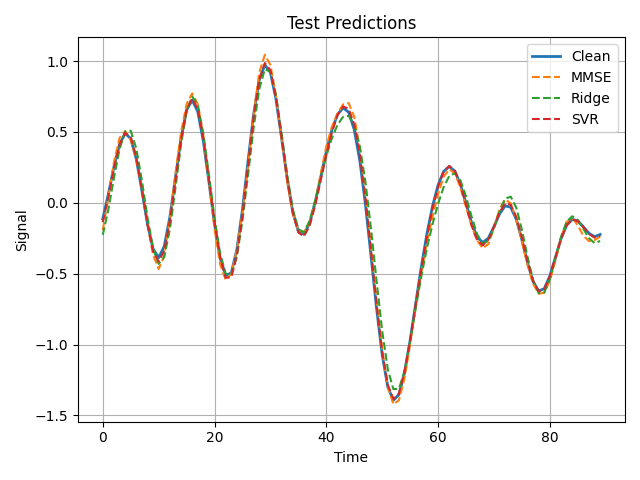
\includegraphics[width=0.5\textwidth]{plots/predictions.png}
			\caption{Clean test signal and predictions from MMSE, Ridge, and SVR.}
			\label{fig:5_1_predictions}
		\end{figure}
		
		\item \textbf{Squared error plots}
		
		We computed the pointwise squared error
		\[
		e_{\text{method}}[n] = \bigl( y_{\text{test,clean}}[n] - \hat{y}_{\text{method}}[n] \bigr)^2
		\]
		for each method. Figure~\ref{fig:5_1_se} shows the squared error over time.
		
		\begin{figure}[H]
			\centering
			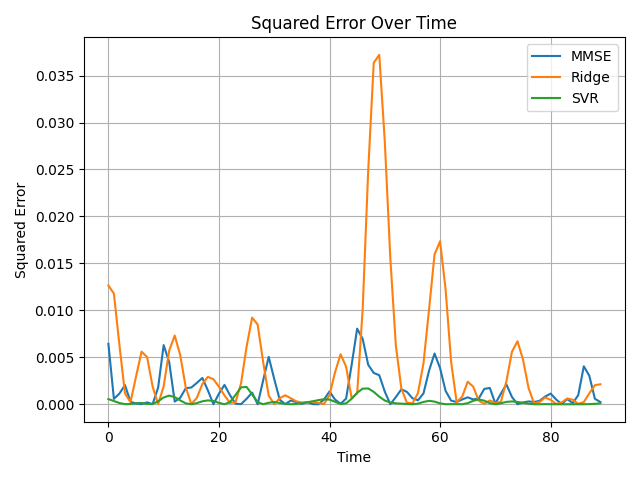
\includegraphics[width=0.5\textwidth]{plots/squared_error.png}
			\caption{Squared error over time for MMSE, Ridge, and SVR.}
			\label{fig:5_1_se}
		\end{figure}
		
		\item \textbf{Discussion of the results}
		
		All three methods track the overall shape of the clean test signal, but their robustness to outliers differs. MMSE,
		which minimizes the mean squared error, is sensitive to large errors in the training targets and shows moderate error
		spikes. Ridge Regression shrinks the weights through the regularization term $\gamma \lVert \mathbf{w} \rVert^2$;
		in this setting it tends to underfit the signal and exhibits the largest squared errors.
		
		SVR, trained with an $\varepsilon$-insensitive loss, is much more robust to outliers in the labels. Small errors
		inside the $\varepsilon$-tube are ignored, and only samples with large residuals become support vectors. As a result,
		SVR achieves the smallest squared error over time and provides the closest approximation to the clean test signal.
	\end{enumerate}
	
	\newpage
	% ---------------- 5.2 ----------------
	\vspace{1em}
	\noindent\textbf{5.2 Performance measures using the correlation coefficient.}
	
	In order to assess the performance of a regressor, a possible measure of performance is the Pearson Correlation Coefficient, which is normalized to 1. Its expression is 
	
	\[
		\rho_{y\hat{y}} = \frac{\mathrm{Cov}(y,\hat{y})}{\sigma_y \,\sigma_{\hat{y}}},
	\]
	
	where $y$ and $\hat{y}$ are the true and predicted signals respectivell. If the prediction is perfect, then, the covariance will be equal to the variance of the signal and the coefficient will be 1. If the prediction does not workj at all, the signals will be uncorrelated, and the covariance will be zero.
	
	\begin{enumerate}[label=\Alph*., leftmargin=1.4cm]
		\item Compute the correlation coefficient of the prediction for different horizons between 1 and 10 between the MMSE soluition and the SRV with the parameters of 5.1. The training regressor will have the same outlier probability and standard deviation as in 5.1.  You may need to repeat the experiment several times and average the results.. The correlation coefficient must be computed with the test regressor without outliers. Explain the results. 
		
		\item Make a graph that shows the correlation between the predictions and the true values by plotting each prediction as a function of the true value, and the identity line superimposed. Do it for H=1 and 5 and for both algorithms. They should have an aspect similar to the one of the figure
		
		\begin{figure}[H]
			\centering
			
\includegraphics[width=0.5\textwidth]{fig_4.png}
		\end{figure}
		
		\item Explain the graphs.
		
		\item Generate a validation set of 100 samples. For H=1 and H=2, construct a crossvalidation loop to select the best possible value of 
		$C$ and $\varepsilon$ for the SVR as a function of the correlation coefficient. You can use the following code to generate the values of both parameters 
		\begin{lstlisting}[style=matlabstyle]
		epsilons = np.logspace(-2, 0, max_epsilons)
		cs       = np.logspace(-2, 2, max_cs)
		\end{lstlisting}
		
		\item Report the optimum values, plot a contour plot of the correlation coefficient as a function of both parameters.
		
		\item Plot a test prediction result for the optimum for both horizons. Comment ther result.
	\end{enumerate}
	
	Link to Google colab code \href{https://colab.research.google.com/drive/14sskFGEKkjr1N7Zq3oHL1NjtsdjTL6zh?usp=sharing}{https://colab.research.google.com/drive/14sskFGEKkjr1N7Zq3oHL1NjtsdjTL6zh?usp=sharing}
	
	\vspace{1em}
	\noindent\textbf{Solution 5.2}
	
	\begin{enumerate}[label=\Alph*., leftmargin=1.4cm]
		
		\item \textbf{Correlation coefficient vs.\ prediction horizon}
		
		For each $H \in \{1,\dots,10\}$ we generated new training and test
		sequences, added outliers to the training targets ($p=0.1$, $a=1$),
		and trained an MMSE regressor and an SVR with $(C=10,
		\varepsilon = 0.01)$. For each horizon we computed the Pearson
		correlation coefficient between the clean test signal and the model
		prediction, averaging over $20$ trials.
		
		The averaged correlation curves in Fig.~\ref{fig:52_corr_vs_horizon}
		show that both models perform almost perfectly for small horizons,
		but SVR degrades much more quickly as $H$ increases. The MMSE model
		stays more stable for longer horizons.
		
		\begin{figure}[H]
			\centering
			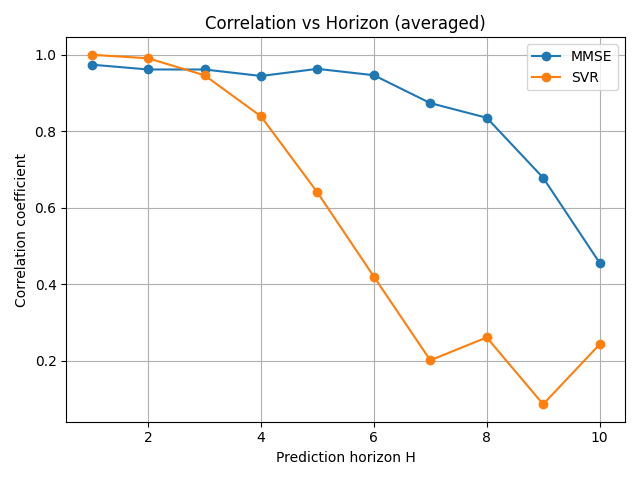
\includegraphics[width=0.6\textwidth]{plots/corr_vs_horizon.png}
			\caption{Average correlation coefficient for MMSE and SVR for
				horizons $H=1$--$10$.}
			\label{fig:52_corr_vs_horizon}
		\end{figure}
		
		\item \textbf{Scatter plots of prediction vs.\ true values}
		
		To visualize how each regressor behaves at different horizons, we
		generated scatter plots for $H = 1$ and $H = 5$. The single combined
		figure (MMSE and SVR for both horizons) is shown in
		Fig.~\ref{fig:52_scatter}.
		
		\begin{figure}[H]
			\centering
			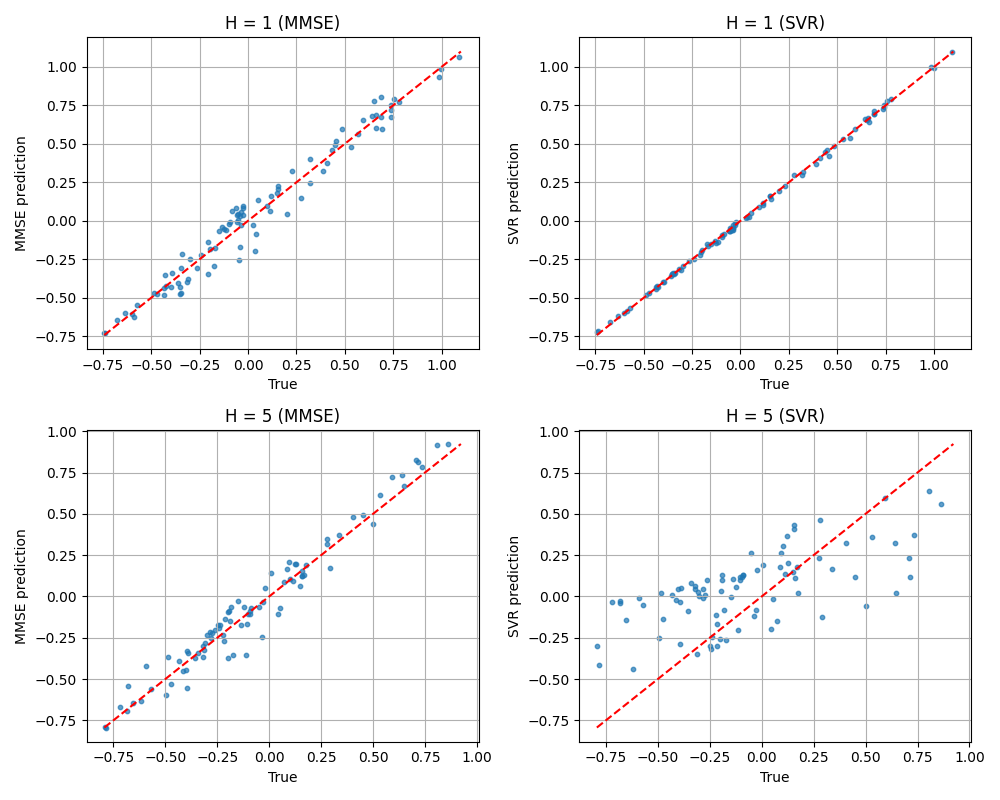
\includegraphics[width=\textwidth]{plots/corr_scatter_H1_H5.png}
			\caption{Scatter plots of prediction vs.\ true values for MMSE and
				SVR at $H=1$ and $H=5$. The identity line is shown in red.}
			\label{fig:52_scatter}
		\end{figure}
		
		\item \textbf{Explanation of the scatter plots}
		
		At $H=1$, both methods land nearly on the identity line, with SVR
		being almost perfectly aligned. At $H=5$, MMSE still roughly tracks
		the structure of the true signal but shows more spread. SVR, on the
		other hand, shows large dispersion and tends to underestimate larger
		values. This aligns with the horizon-dependent correlations in part~A.
		
		\item \textbf{Cross-validation over $C$ and $\varepsilon$}
		
		We performed a grid search over
		\begin{lstlisting}[style=matlabstyle]
	epsilons = np.logspace(-2, 0, max_epsilons)
	cs       = np.logspace(-2, 2, max_cs)
		\end{lstlisting}
		using a clean validation sequence. The correlation maps for $H=1$
		and $H=2$ are shown together in
		Fig.~\ref{fig:52_contour_combined}. In both cases, the best
		performance occurs at a small $\varepsilon$ and large $C$, with the
		optimal values
		\[
		\varepsilon^\star = 0.01, \qquad C^\star = 100.
		\]
		
		\begin{figure}[H]
			\centering
			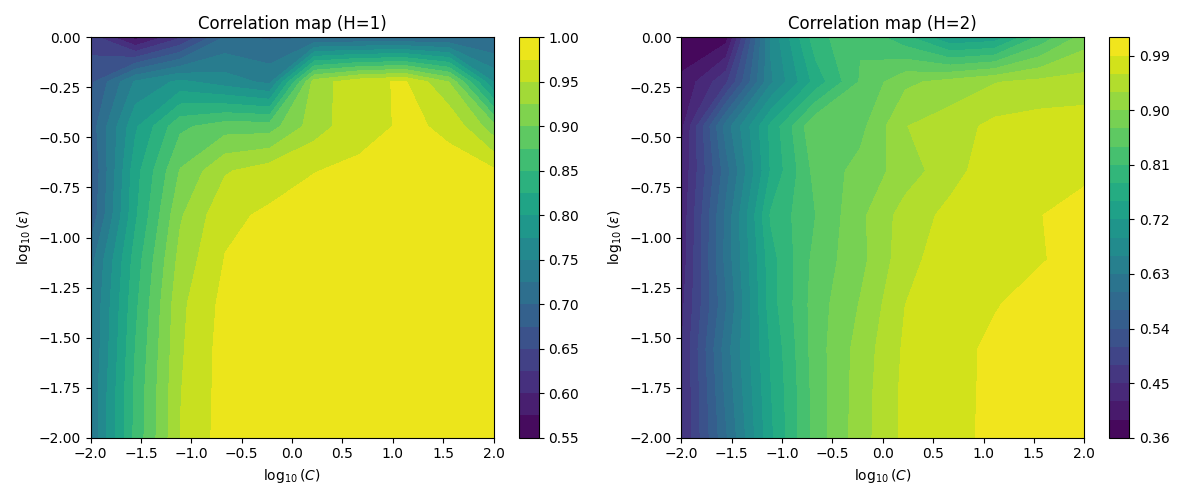
\includegraphics[width=\textwidth]{plots/contour_corr_combined.png}
			\caption{Validation correlation maps for $(C,\varepsilon)$ for
				$H=1$ (left) and $H=2$ (right).}
			\label{fig:52_contour_combined}
		\end{figure}
		
		\item \textbf{Test performance with optimal parameters}
		
		Using the optimal hyperparameters above, we retrained the SVR and
		evaluated it on the clean test signal. The test correlations were
		
		\begin{center}
			\begin{tabular}{c|c|c}
				Horizon $H$ & $\varepsilon^\star$ & Test Correlation $\rho$ \\
				\hline
				1 & 0.01 & 0.9999 \\
				2 & 0.01 & 0.9981 \\
			\end{tabular}
		\end{center}
		
		The corresponding predictions (side-by-side) are shown in
		Fig.~\ref{fig:52_pred_best}.
		
		\begin{figure}[H]
			\centering
			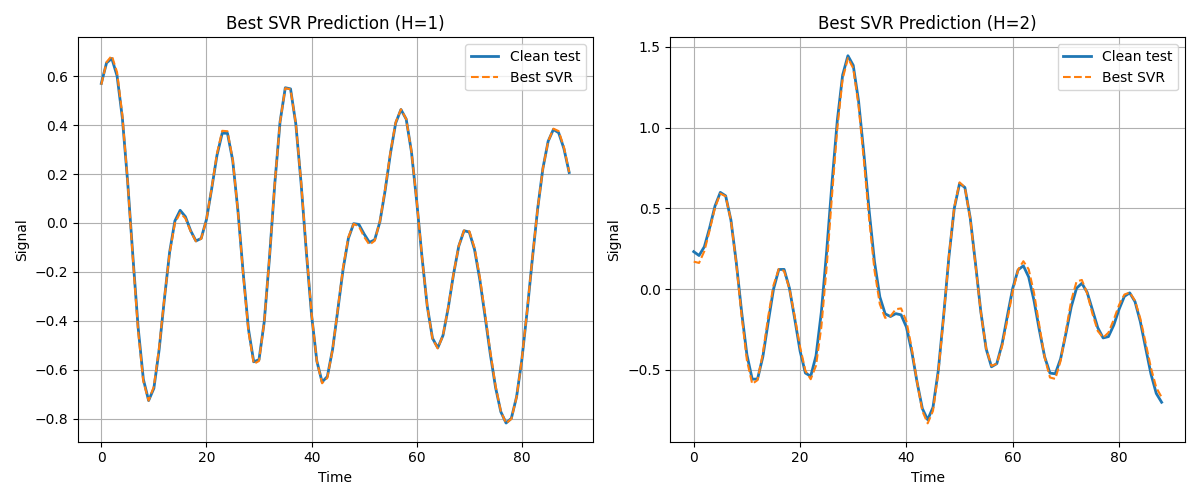
\includegraphics[width=\textwidth]{plots/pred_best_SVR.png}
			\caption{Best SVR predictions for $H=1$ (left) and $H=2$ (right).}
			\label{fig:52_pred_best}
		\end{figure}
		
		\item \textbf{Comment on the results}
		
		SVR performs extremely well for short-term prediction when $C$ is
		large and $\varepsilon$ is small—essentially matching the clean test
		signal at $H=1$. However, as the horizon increases, SVR becomes more
		sensitive to outliers and the inherent difficulty of multi-step
		prediction, while the MMSE regressor degrades much more gradually.
		This makes MMSE more reliable for longer-term forecasts in this
		setting.
		
	\end{enumerate}
	
	\newpage
	
	\begin{lstlisting}[style=matlabstyle]
from scipy import signal
import matplotlib.pyplot as plt
from sklearn.svm import SVR
import numpy as np
import os

os.makedirs("plots", exist_ok=True)
np.random.seed(0)

def buffer(x, n, hop):  # Generated with AI. This returns an array of buffered signal windows
"""
Args:
x: Input array.
n: Length of each buffer.
hop: Hop size (The overlap is n-hop).

Returns:
A 2D array where each row is a buffer.
"""
if len(x) < n:
raise ValueError("Input array length must be greater than or equal to the buffer length.")
num_buffers = (len(x) - n) // hop + 1
result = np.zeros((num_buffers, n))
for i in range(num_buffers):
start = i * hop
end = start + n
result[i, :] = x[start:end]
return result

def signal_gen(sigma, N):
T = 200
sos = signal.butter(10, 0.2, 'low', output='sos')
z = np.random.randn(N+T)
x = signal.sosfilt(sos, z)
x = x + sigma*np.random.randn(x.shape[0])
x = x[T:]
return x

def add_outliers(x, p, a):
x = x + a*(np.random.rand(x.shape[0]) > (1-p))*np.random.randn(x.shape[0])
return x

def build_datasets(N=100, W=10, H=1, sigma=0.0):
xtrain = signal_gen(sigma, N)
xval   = signal_gen(sigma, N)
xtest  = signal_gen(sigma, N)

Xtrain_full = buffer(xtrain, W, 1)
Xval_full   = buffer(xval,   W, 1)
Xtest_full  = buffer(xtest,  W, 1)

ytrain_clean = xtrain[W+H-1:]
yval_clean   = xval[W+H-1:]
ytest_clean  = xtest[W+H-1:]

Xtrain = Xtrain_full[0:-H]
Xval   = Xval_full[0:-H]
Xtest  = Xtest_full[0:-H]

return Xtrain, ytrain_clean, Xval, yval_clean, Xtest, ytest_clean

def corrcoef(y_true, y_pred):
return np.corrcoef(y_true, y_pred)[0, 1]

N = 100
W = 10
H = 1
sigma = 0.0

xtrain = signal_gen(sigma, N)
xtest  = signal_gen(sigma, N)

Xtrain_full = buffer(xtrain, W, 1)
ytrain_clean = xtrain[W+H-1:]
Xtrain = Xtrain_full[0:-H]

print("\n5.1A")
print("Xtrain shape:", Xtrain.shape)
print("ytrain_clean shape:", ytrain_clean.shape)

Xtest_full = buffer(xtest, W, 1)
ytest_clean = xtest[W+H-1:]
Xtest = Xtest_full[0:-H]

print("Xtest shape:", Xtest.shape)
print("ytest_clean shape:", ytest_clean.shape)

p = 0.1
a = 1.0
ytrain = add_outliers(ytrain_clean.copy(), p, a)

X = Xtrain.T
y = ytrain
XXT = X @ X.T
Xy = X @ y

w_mmse = np.linalg.solve(XXT, Xy)
w_ridge = np.linalg.solve(XXT + 0.2*np.eye(XXT.shape[0]), Xy)

svr_model = SVR(C=10.0, epsilon=0.01, kernel='linear')
svr_model.fit(Xtrain, ytrain)

yhat_mmse  = Xtest @ w_mmse
yhat_ridge = Xtest @ w_ridge
yhat_svr   = svr_model.predict(Xtest)

print("\n5.1B")
print("Models trained: MMSE, Ridge, SVR")

t = np.arange(len(ytest_clean))
plt.figure()
plt.plot(t, ytest_clean, label='Clean', linewidth=2)
plt.plot(t, yhat_mmse,  '--', label='MMSE')
plt.plot(t, yhat_ridge, '--', label='Ridge')
plt.plot(t, yhat_svr,   '--', label='SVR')
plt.xlabel('Time')
plt.ylabel('Signal')
plt.title('Test Predictions')
plt.grid()
plt.legend()
plt.tight_layout()
plt.savefig("plots/predictions.png")
plt.close()
print("5.1C: saved plots/predictions.png")

# 5.1D
se_mmse  = (ytest_clean - yhat_mmse)**2
se_ridge = (ytest_clean - yhat_ridge)**2
se_svr   = (ytest_clean - yhat_svr)**2

plt.figure()
plt.plot(t, se_mmse,  label='MMSE')
plt.plot(t, se_ridge, label='Ridge')
plt.plot(t, se_svr,   label='SVR')
plt.xlabel('Time')
plt.ylabel('Squared Error')
plt.title('Squared Error Over Time')
plt.grid()
plt.legend()
plt.tight_layout()
plt.savefig("plots/squared_error.png")
plt.close()
print("5.1D: saved plots/squared_error.png")

print("\n5.2A")

p = 0.1
a = 1.0
W = 10
sigma = 0.0
N = 100
num_trials = 20
Hs = np.arange(1, 11)

corr_mmse = np.zeros_like(Hs, dtype=float)
corr_svr  = np.zeros_like(Hs, dtype=float)

for idx, H in enumerate(Hs):
cm = []
cs = []
for _ in range(num_trials):
Xtrain, ytrain_clean, _, _, Xtest, ytest_clean = build_datasets(N, W, H, sigma)
ytrain = add_outliers(ytrain_clean.copy(), p, a)

X = Xtrain.T
y = ytrain
XXT = X @ X.T
Xy  = X @ y

w_mmse = np.linalg.solve(XXT, Xy)
yhat_mmse = Xtest @ w_mmse

svr = SVR(C=10.0, epsilon=0.01, kernel='linear')
svr.fit(Xtrain, ytrain)
yhat_svr = svr.predict(Xtest)

cm.append(corrcoef(ytest_clean, yhat_mmse))
cs.append(corrcoef(ytest_clean, yhat_svr))

corr_mmse[idx] = np.mean(cm)
corr_svr[idx]  = np.mean(cs)

plt.figure()
plt.plot(Hs, corr_mmse, 'o-', label='MMSE')
plt.plot(Hs, corr_svr,  'o-', label='SVR')
plt.xlabel('Prediction horizon H')
plt.ylabel('Correlation coefficient')
plt.title('Correlation vs Horizon (averaged)')
plt.grid()
plt.legend()
plt.tight_layout()
plt.savefig("plots/corr_vs_horizon.png")
plt.close()
print("5.2A: saved plots/corr_vs_horizon.png")

print("\n5.2B")

def get_run(H):
Xtrain, ytrain_clean, _, _, Xtest, ytest_clean = build_datasets(N, W, H, sigma)
ytrain = add_outliers(ytrain_clean.copy(), p, a)

X = Xtrain.T
y = ytrain
XXT = X @ X.T
Xy  = X @ y
w_mmse = np.linalg.solve(XXT, Xy)
yhat_mmse = Xtest @ w_mmse

svr = SVR(C=10.0, epsilon=0.01, kernel='linear')
svr.fit(Xtrain, ytrain)
yhat_svr = svr.predict(Xtest)

return ytest_clean, yhat_mmse, yhat_svr

Hs_scatter = [1, 5]

plt.figure(figsize=(10,8))
for i, H in enumerate(Hs_scatter, 1):
ytrue, yhat_m, yhat_s = get_run(H)
ymin = min(ytrue.min(), yhat_m.min(), yhat_s.min())
ymax = max(ytrue.max(), yhat_m.max(), yhat_s.max())
line = np.linspace(ymin, ymax, 100)

plt.subplot(2,2,2*i-1)
plt.scatter(ytrue, yhat_m, s=10, alpha=0.7)
plt.plot(line, line, 'r--')
plt.xlabel('True')
plt.ylabel('MMSE prediction')
plt.title(f'H = {H} (MMSE)')
plt.grid()

plt.subplot(2,2,2*i)
plt.scatter(ytrue, yhat_s, s=10, alpha=0.7)
plt.plot(line, line, 'r--')
plt.xlabel('True')
plt.ylabel('SVR prediction')
plt.title(f'H = {H} (SVR)')
plt.grid()

plt.tight_layout()
plt.savefig("plots/corr_scatter_H1_H5.png")
plt.close()
print("5.2B: saved plots/corr_scatter_H1_H5.png")

print("\n5.2D-F")

def svr_grid_search(H, epsilons, cs):
Xtrain, ytrain_clean, Xval, yval_clean, Xtest, ytest_clean = build_datasets(N, W, H, sigma)
ytrain = add_outliers(ytrain_clean.copy(), p, a)

corr_grid = np.zeros((len(epsilons), len(cs)))
for i, eps in enumerate(epsilons):
for j, C in enumerate(cs):
svr = SVR(C=C, epsilon=eps, kernel='linear')
svr.fit(Xtrain, ytrain)
yhat_val = svr.predict(Xval)
corr_grid[i, j] = corrcoef(yval_clean, yhat_val)

best_idx = np.unravel_index(np.argmax(corr_grid), corr_grid.shape)
best_eps = epsilons[best_idx[0]]
best_C   = cs[best_idx[1]]

svr_best = SVR(C=best_C, epsilon=best_eps, kernel='linear')
svr_best.fit(Xtrain, ytrain)
yhat_test = svr_best.predict(Xtest)
corr_test = corrcoef(ytest_clean, yhat_test)

return Xtrain, ytrain_clean, Xval, yval_clean, Xtest, ytest_clean, corr_grid, best_eps, best_C, yhat_test, corr_test

max_epsilons = 10
max_cs = 10
epsilons = np.logspace(-2, 0, max_epsilons)
cs       = np.logspace(-2, 2, max_cs)

pred_results = {}
contour_data = {}

for H in [1, 2]:
print(f"\nH = {H}")
(Xtrain, ytrain_clean, Xval, yval_clean,
Xtest, ytest_clean, corr_grid, best_eps, best_C,
yhat_test, corr_test) = svr_grid_search(H, epsilons, cs)

print(f"Best epsilon: {best_eps:.4f}, Best C: {best_C:.4f}, Test corr: {corr_test:.4f}")

contour_data[H] = corr_grid
pred_results[H] = (ytest_clean, yhat_test)

Xg, Yg = np.meshgrid(np.log10(cs), np.log10(epsilons))
plt.figure(figsize=(12,5))

for i, H in enumerate([1, 2], 1):
plt.subplot(1, 2, i)
cp = plt.contourf(Xg, Yg, contour_data[H], levels=20)
plt.colorbar(cp)
plt.xlabel(r'$\log_{10}(C)$')
plt.ylabel(r'$\log_{10}(\varepsilon)$')
plt.title(f'Correlation map (H={H})')
plt.grid(False)

plt.tight_layout()
plt.savefig("plots/contour_corr_combined.png")
plt.close()
print("Saved plots/contour_corr_combined.png")

print("\nSaving combined best-SVR test predictions...")

plt.figure(figsize=(12,5))

for i, H in enumerate([1, 2], 1):
ytrue, yhat_best = pred_results[H]
t = np.arange(len(ytrue))

plt.subplot(1, 2, i)
plt.plot(t, ytrue, label='Clean test', linewidth=2)
plt.plot(t, yhat_best, '--', label='Best SVR')
plt.xlabel("Time")
plt.ylabel("Signal")
plt.title(f"Best SVR Prediction (H={H})")
plt.grid()
plt.legend()

plt.tight_layout()
plt.savefig("plots/pred_best_SVR.png")
plt.close()

print("Saved plots/pred_best_SVR.png")
	\end{lstlisting}
\end{document}
